%
% Szakdolgozatminta az Eszterházy Károly Katolikus Egyetem
% matematika illetve informatika szakos hallgatóinak.
%

\documentclass[
% opciók nélkül: egyoldalas nyomtatás, elektronikus verzió
% twoside,     % kétoldalas nyomtatás
% tocnopagenum,% oldalszámozás a tartalomjegyzék után kezdődik
]{thesis-ekf}
\usepackage[T1]{fontenc}
\PassOptionsToPackage{defaults=hu-min}{magyar.ldf}
\usepackage[magyar]{babel}
\usepackage{mathtools,amssymb,amsthm,pdfpages,listingsutf8,xurl}

\footnotestyle{rule=fourth}

\newtheorem{tetel}{Tétel}[chapter]
\theoremstyle{definition}
\newtheorem{definicio}[tetel]{Definíció}
\theoremstyle{remark}
\newtheorem{megjegyzes}[tetel]{Megjegyzés}

\lstset{
    language=[Sharp]C,
    inputencoding=utf8/latin2,
    basicstyle=\footnotesize\ttfamily,
    columns=fullflexible,
    numbers=left,
    breaklines,
    xleftmargin=0.7cm,
    xrightmargin=0.7cm,
    frame=ltrb,
    rulecolor=\color{blue!80!black},
    backgroundcolor=\color{gray!30},
    commentstyle=\color{green!60!black},
    keywordstyle=\color{blue},
    morekeywords={using,public,class,int,void,new,for,bool,false,true,if},
}
\renewcommand{\lstlistingname}{kód}

\begin{document}

\institute{Matematikai és Informatikai Intézet}
\title{A szakdolgozat címe}
\author{Pataki Tamás\\Programtervező Informatikus BSc}
\supervisor{Tanár neve\\beosztás}
\city{Eger}
\date{2024}
\maketitle

\tableofcontents

\chapter*{Bevezetés}
\addcontentsline{toc}{chapter}{Bevezetés}
A szakdolgozati a téma választás idején sok lehetőség közül lehetett választanom.
Végül amikor választnom kellet olyan témát szerettem volna amely egy sajátos kiívást és egyben az érdekeltségi közömbe is tartozik téma szerint.
A játékfejlesztés érdekelt korábban is, 

Ezek a faktorok alapján választottam játék fejlesztést Unity\cite{Unity} játékmotorral, melyben a fejlesztész C\# programozási nyelven alapszik. A 3D projekt mellet döntöttem, ez felelt meg az elképzeléseimhez. 

\chapter{Felhasznált technológiák}

\section{Unity}

A fejlesztésem alapjának a Unity-t választottam népszerűsége és sokoldalúsága miatt. Rengeteg eszközt ad a fejlesztő kezébe, így szinte bármilyen típusú projektet lehet vele készíteni, akár a játékfejlesztésen túl is.

\subsection{A Unity-ről általánosan}

A projektek Unity-ben több jelenetből (scene-ből) épülnek fel, melyek tartalmaznak Gameobjecteket.

\subsection{Gameobject-ek}

Egyik alapeleme a Unity-nek a GameObjectek, melyeknek rengeteg féle felhasználási módjuk van. Bármilyen karakter, pálya vagy tárgy egy Gameobject egy jeleneten belül.
Alapból nincsen konkrét funkciójúk, de komponenseket lehet hozzájuk csatolni, melyek meghatározzás a működésüket. Az egyik alap komponen a Transform, mely minden gameobject-nek van, és a pozíciót, forgatást és méretet kezeli.



\subsection{Scene-k}


\subsection{Szkriptelés}

A szkriptek egyféle komponens a Gameobjectnek. A játék logikájának és interakcióinak megírására szolgálnak. A szkriptek főként C\# nyelven készülnek, és az egyes játékobjektumok viselkedését, mozgását, valamint a játékbeli eseményeket szabályozzák.


A Monobehavior-ből nevű osztályból öröklődik a legtöbb szkript, mely többféle életciklus metódust:

\begin{itemize}
    \item Start
    \item Update
    \item FixedUpdate
    \item OnCollisionEnter / OnTriggerEnter
\end{itemize}

A Start metódus egyszer fut le a szkript indításakor, amikor a jelenet betöltődik, és az objektum engedélyezve van. Általában inicializálási feladatokat, például változók értékeinek beállítását hajtja végre.
\\
Az Update metódus minden képkockánál lefut, így ide kerülnek azok a kódok, amelyeknek folyamatosan, valós időben kell futniuk, például kamerakövetés.

A FixedUpdate, az Update-hez hasonlóan, folyamatosan fut, viszont minden fizikai képkockán fut le, a megjelenített képkockáktől függetlenul. Ide a fizikai számítások kerülnek.

Az OnCollisionEnter akkor fut le amikor két tárgy amelyek van Collider-e összeütközik. Ezt

\subsection{Prefab-ek}



\section{Blender}

A modellezéshez Blendert választottam a tág eszközkészlete és sok tanulási anyaga miatt.


\chapter{A játék bemutatása}


\section{A játékmenet}

A fő eleme a játéknak a Tank részeinek kiválasztásának a lehetősége, melyet a főmenüben lehetséges.
\subsection{Tank kiválasztása}

\subsection{Csata}



\section{A megvalósítás}

\subsection{A tank}

A tank komponens sok dologért felel. Legfőként a különböző részek létrehozásáért, statisztikáiknak az összekombinálásáért és az életerő kezeléséért felel.
\lstinputlisting[caption=A tank létrehozása,label=tankspawn]{./codesnippets/tankspawn.cs}

Ez a komponens egyéni tapadási fizikáért is felel, mely gyorsabb sebességnél történő fordulásnál nagy mértékben csökkenti a tank sebességét és a fordulás irányába viszi a tankot. Ennek hiányában forduláskor nem lenne tapadás és oldalirányban tudna csúszni.

\lstinputlisting[caption=Torony irányítása,label=tracion]{./codesnippets/traction.cs}


A tank 3 részre van felosztva:
\begin{itemize}
    \item Tanktest
    \item Torony
    \item Ágyú
\end{itemize}




\subsubsection{Páncélzati rendszer}
Minden tank modellje fel van osztva több kis darabra, melynek van a beépített Collider komponense és a saját páncél komponense. Ezzel a módszerrel pontosan meg lehet adni hogy mely részen mekkora védelme van és mekkora sebzési szorzót kap. Például az ágyúnak és a lánctalpnak kisebb szorzója van, mivel könnyebben átüthető részeknek számítanak, miközben a tank középpontja nem kap sebzést.

\subsubsection{Tanktest}

Ez a rész adja meg az egész tank teljes sebességét, gyorsulását, a motor hangját és az életerejének a nagy részét. Valamint hozzá tartoznak a lánctalpak is, melyek ellenőrzik, hogy a tank a földön van-e egy adott pillanatban egy rövid sugár segítségével, mely megnézi hogy a terep-be ütközött-e be.  Általánosan ez rendelkezik a legtöbb páncél elemmel is.

\subsubsection{Torony}

A torony forgatását egy

\lstinputlisting[caption=Torony irányítása,label=turretrotation]{./codesnippets/turretrotation.cs}

\subsubsection{Ágyú}

A torony forgatásához hasonlóan a cső is egy üres játék objektum használ, mely felé

\lstinputlisting[caption=Torony irányítása,label=barrelelevation]{./codesnippets/barrelelevation.cs}


\subsubsection{Irányítás}



\subsubsection{Célzás}

\subsubsection{Játékos nézőpontja}

A játékos nézőpontja 2 darab kamerával van megoldva, külső és belső nézetes, melyeknek az érzékenységét külön lehet beállítani.

\subsection{Menü}


\subsubsection{Tank kiválasztása}

A kiválasztási menüben a felső részen a gombok segítségével választhatóak a tank részei, és a gombok között található azoknak a megnevezése. A jobb alsó sarokban található a játék indító gomb, mely indítja a játékmenetet.

\subsubsection{Beállítások}

A beállításokban az érzékenységet és a hangerőt lehet állítani, melyeknek

\subsubsection{Szünet menü}

Egy egyszerűbb szünet menü van a játékban, mellyel újralehet indítani a játékmenetet vagy visszamenni a fő menübe. Ilyenkor a játékmenet teljesen megáll illetve a kurzor újra látható és mozgathatóvá válik.

\subsection{Irányítás bevitele}

A bevitelhez a Unity új beviteli rendszerét használtam segítségül.


\subsection{Lövedékek}

A lövedékek fizikai objektumként működnek,

Három féle lövedék van beimplementálva jelenleg a játékba:
\begin{itemize}
    \item páncéltörő
    \item robbanótöltetes pácéltörő
    \item robbanótöltet
\end{itemize}

\lstinputlisting[caption=Torony irányítása,label=bullet]{./codesnippets/bullet.cs}

Ezekből a változók beállításával lehet további típusokat beállítani.

\subsubsection{Páncéltörő lövedék}

A páncél törő lövedék a DeMarr formula alapján lett modellezve. Ez adja meg a súly, átmérő és sebesség alapján az alap átütési erejét egy adott lövedéknek.

%DeMarr Formula
\begin{equation}
 P_r \times (\frac{V}{V_r})^{1,4283} \times ( \frac{D}{D_r})^{1,0714}  \times \frac{(\frac{W}{\varnothing})^{0,7143}}{(\frac{W_r}{\varnothing_r})^{0,7143}}
\end{equation}

Ezentúl a lövdéknek a megtett távolsága és a találat szöge is figyelmbe van véve. Ezek befolyásának a mértékét kettő változóval lehet állítani. A távolságnál az 1-es érték figyelmen kívűl hagyja a szorzót, az 1 alatti érték, melyet a legtöbb lövedék használ, nagyobb távolságnál csökkenti az átütés mértékét, míg az 1 feletti érték növeli. A szögteljesíménynél az 0-ás érték nem veszi figyelmbe a szög mértékét, az 1-es érték a páncélvastagságnak $\cos$ értékét nézi, mely egyenlő az adott szög alapján figyelmebe vett vastagságával és a leggyakrabban használt 1 feletti érték gyengíti nagyobb szög esetén. Ha a távolsági és a szögteljesíményi értékeket 1-re állítjuk akkor egy másfajta lövedék típust lehet elérni.

\lstinputlisting[caption=Átütés kiszámítása,label=APcalculation]{./codesnippets/APcalculation.cs}

\subsubsection{Robbanótöltetes lövedék}

Az alábbi lövedék egy felülethez érvén egy robbanást olyan módon utánoz hogy a megadott átmérőjű gömbön belül először megnézni az összes objektum között hogy bármyelik páncélnak számít-e, majd a robbanás középpontjától számítva mely páncéllemeznek a legkevesebb a vastagsága és a távolságának a keveréke.

\lstinputlisting[caption=Torony irányítása,label=hexplosion]{./codesnippets/heexplosion.cs}

\subsubsection{Robbabótöltetes páncéltörő lövedék}

Ez a lövedék hasonlóan működik a

\subsection{Kezelő felület}

\subsubsection{Életerő csík}

Két féle életerő csík létezik a projektben. Az egyik a kezelő felületen fixen található a bal alsó sarokba, ez kijelzi a teljes és a jelenlegi életerőt számmal, illetve hiányzó életerő szerint kevesebb része lesz kitöltve. A másik az ellenfelek felett megtalálható, és a 3D térben helyezkednek ell

\subsubsection{Célkereszt}

A cél kereszt 2 részből áll. A kör alakú irányzék a képernyő közepét és a kívánt célpontot jelzi, emellett lövés után pirossá változik, jelezve az újratöltés menetét. A második, kereszt alakú, pedig azt jelzi, hogy a cső jelenleg milyen irányba néz.

\begin{figure}[h]
    \centering
    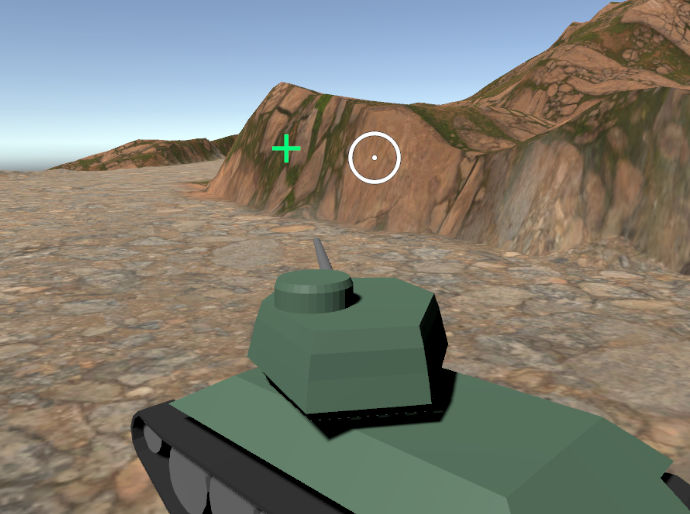
\includegraphics[width=0.5\textwidth]{screenshots/crosshair.png}
    \caption{Célkeresztek}
    \label{fig:crosshair}
\end{figure}

\subsection{Ellenfelek}

\subsubsection{Navmesh}

Az ellenfelek útkeresését a Unity-nak a beépített Navmesh rendszere segítségével oldottam meg.

\subsubsection{Ellenőrző pontok}

Az ellefeleknek van egy megadott útvonaluk amit követnek, melyet ellenőrző pontok segítségével oldottam meg.

%\lstinputlisting[caption=Torony irányítása,label=checkpoints]{./codesnippets/checkpointsystem.cs}

\subsubsection{Állapotgép}

Állaptgép használatával van megoldva az ellenfelek viselkedésének szétválasztása. Azért választottam állapotgépet ehhez, mert egy tiszta és egyszerűen bővíthető módszert ad különböző viselkedések és állapotok megadására.

\lstinputlisting[caption=Torony irányítása,label=statemachine]{./codesnippets/statemachine.cs}

\subsubsection{Állapotok}

Kétféle állapot van:
\begin{itemize}
 \item Járőrözés
 \item Támadás
\end{itemize}

\subsubsection{Járőrözés}

\subsubsection{Támadás}

\lstinputlisting[caption=Állapotgép,label=checkplayervisible]{./codesnippets/checkplayervisible.cs}

\chapter{Tesztelés}

\chapter*{Összegzés}

\addcontentsline{toc}{chapter}{\bibname}

\begin{thebibliography}{55}
    \bibitem{Unity}
    \textsc{Unity} \emph{Unity Documentation}
    \\
    \url{https://docs.unity.com/}



\end{thebibliography}

\end{document}
